

\tikzset{every picture/.style={line width=0.75pt}} %set default line width to 0.75pt        

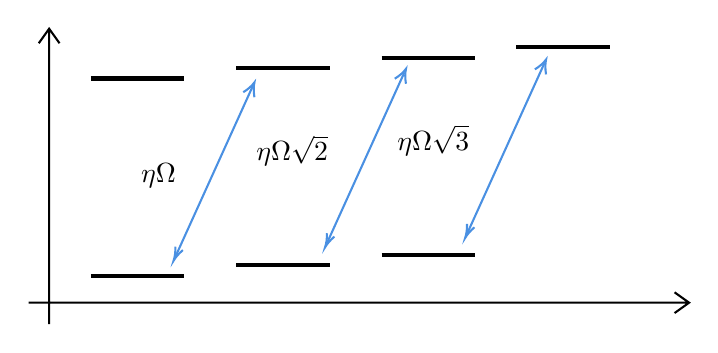
\begin{tikzpicture}[x=0.75pt,y=0.75pt,yscale=-1,xscale=1]
%uncomment if require: \path (0,158); %set diagram left start at 0, and has height of 158

%Shape: Axis 2D [id:dp15618946884319262] 
\draw  (0,138) -- (318.17,138)(9.85,6) -- (9.85,148.38) (311.17,133) -- (318.17,138) -- (311.17,143) (4.85,13) -- (9.85,6) -- (14.85,13)  ;
%Straight Lines [id:da5633161593663423] 
\draw [line width=1.5]    (30,125) -- (75,125) ;
%Straight Lines [id:da6891482979787938] 
\draw [color={rgb, 255:red, 74; green, 144; blue, 226 }  ,draw opacity=1 ]   (107.95,33.65) -- (70.6,116.01) ;
\draw [shift={(69.77,117.83)}, rotate = 294.39] [color={rgb, 255:red, 74; green, 144; blue, 226 }  ,draw opacity=1 ][line width=0.75]    (6.56,-1.97) .. controls (4.17,-0.84) and (1.99,-0.18) .. (0,0) .. controls (1.99,0.18) and (4.17,0.84) .. (6.56,1.97)   ;
\draw [shift={(108.77,31.83)}, rotate = 114.39] [color={rgb, 255:red, 74; green, 144; blue, 226 }  ,draw opacity=1 ][line width=0.75]    (6.56,-2.94) .. controls (4.17,-1.38) and (1.99,-0.4) .. (0,0) .. controls (1.99,0.4) and (4.17,1.38) .. (6.56,2.94)   ;
%Straight Lines [id:da5552335178166578] 
\draw [line width=1.5]    (30,30) -- (75,30) ;
%Straight Lines [id:da6891740634193314] 
\draw [line width=1.5]    (100,120) -- (145,120) ;
%Straight Lines [id:da5661851604865566] 
\draw [line width=1.5]    (100,25) -- (145,25) ;
%Straight Lines [id:da6022612634715885] 
\draw [line width=1.5]    (170,115) -- (215,115) ;
%Straight Lines [id:da9393350496146184] 
\draw [line width=1.5]    (170,20) -- (215,20) ;
%Straight Lines [id:da2934899407823195] 
\draw [line width=1.5]    (235,15) -- (280,15) ;
%Straight Lines [id:da3308284960238893] 
\draw [color={rgb, 255:red, 74; green, 144; blue, 226 }  ,draw opacity=1 ]   (180.95,27.15) -- (143.6,109.51) ;
\draw [shift={(142.77,111.33)}, rotate = 294.39] [color={rgb, 255:red, 74; green, 144; blue, 226 }  ,draw opacity=1 ][line width=0.75]    (6.56,-1.97) .. controls (4.17,-0.84) and (1.99,-0.18) .. (0,0) .. controls (1.99,0.18) and (4.17,0.84) .. (6.56,1.97)   ;
\draw [shift={(181.77,25.33)}, rotate = 114.39] [color={rgb, 255:red, 74; green, 144; blue, 226 }  ,draw opacity=1 ][line width=0.75]    (6.56,-2.94) .. controls (4.17,-1.38) and (1.99,-0.4) .. (0,0) .. controls (1.99,0.4) and (4.17,1.38) .. (6.56,2.94)   ;
%Straight Lines [id:da6178275915895299] 
\draw [color={rgb, 255:red, 74; green, 144; blue, 226 }  ,draw opacity=1 ]   (248.45,22.65) -- (211.1,105.01) ;
\draw [shift={(210.27,106.83)}, rotate = 294.39] [color={rgb, 255:red, 74; green, 144; blue, 226 }  ,draw opacity=1 ][line width=0.75]    (6.56,-1.97) .. controls (4.17,-0.84) and (1.99,-0.18) .. (0,0) .. controls (1.99,0.18) and (4.17,0.84) .. (6.56,1.97)   ;
\draw [shift={(249.27,20.83)}, rotate = 114.39] [color={rgb, 255:red, 74; green, 144; blue, 226 }  ,draw opacity=1 ][line width=0.75]    (6.56,-2.94) .. controls (4.17,-1.38) and (1.99,-0.4) .. (0,0) .. controls (1.99,0.4) and (4.17,1.38) .. (6.56,2.94)   ;

% Text Node
\draw (52.67,69.46) node [anchor=north west][inner sep=0.75pt]    {$\eta\Omega $};
% Text Node
\draw (108.17,55.96) node [anchor=north west][inner sep=0.75pt]    {$\eta\Omega \sqrt{2}$};
% Text Node
\draw (176.17,50.96) node [anchor=north west][inner sep=0.75pt]    {$\eta\Omega \sqrt{3}$};


\end{tikzpicture}
